\chapter{GAMs with stratified smoothers and PMSD tests}



%	\title{A Stratified Generalized Additive Model and Permutation Test for Temporal Heterogeneity of Smoothed Bivariate Spatial Effects}
	
	\section{Introduction}
	
	Spatial differences in disease risk are potential indicators of space-related disease factors such as environmental exposures or availability of sufficient health care in certain areas. As such, quantification of heterogeneity in disease risk patterns over geographical space is of common interest in epidemiology studies. 
	
	While traditional geographic modeling methods focus on analyzing aggregated area-level data that treat area-defined partitions as one unit, more recent spatial epidemiology studies avoid aggregation bias and ecological fallacy by modeling individual-level data.  With accurate records of geospatial information over a  period of time, researchers seek to draw inference on both the existence of spatial effects on risks of disease as well as potential changes in spatial patterns of disease over time. As one example, \cite{girguis2016maternal} conducted a fairly recent study of birth defects in the state of Massachusetts.  In the study, all recorded births in the Massachusetts Birth Defects Registry (MBDR) having cardiac, orofacial and neural tube defects from 2001 to 2009 were identified as cases and 1000 live births per year without defects were sampled as common controls. Among the birth defects considered in the case definition, one of the most common was patent ductus arteriosus (PDA).  PDA is a cardiovascular birth defect in which abnormal blood flow occurs between two of the major arteries connected to the heart and is associated with high morbidity and mortality. Residential longitude and latitude were recorded for all observations as well as potential confounding variables including maternal age, adequacy of prenatal care (measured by the Adequacy of Prenatal Care Utilization Index), maternal race, maternal education level and number of siblings. 
	
	A primary goal of the MBDR study is to quantify geospatial risks for PDA, after adjusting for known risk factors. It is not generally  reasonable to assume an \emph{a priori}  parametric form on spatial effects, as spatial disease patterns are often complex and require flexible modeling techniques. Because of this, smoothers are commonly used in such settings. In spatial analyses, smoothers consider the underlying spatial risk pattern as a flexible bivariate function of $(u,v)$, the longitude and latitude associated with a given response. Popular smoothers for spatial risk pattern estimation generally belong to two broad categories: kernel smoothers and spline smoothers. \cite{hastie1990generalized} introduced both categories and consider the incorporation of the smoothing techniques into regression-based methods otherwise known as generalized additive models (GAMs). \cite{wood2017generalized} focused on spline smoothers and offered a full introduction to knot-based splines, smoothing splines and regression splines.  %Splines are developed by placing knots at various points in the support of the predictor space and fitting piecewise parametric models between each set of knots. Constraints are then used to ensure some degree of smoothness at the knot locations.  
	
	Popular smoothing functions for geographical analysis include local weighted scatterplot smoothing (LOESS) and thin-plate regression splines. LOESS was first proposed by \cite{cleveland1979robust} for flexible smoothing with moving weighted linear regressions. LOESS assumes local (weighted) linearity, resulting in flexible functional estimation for the whole domain. The method was further applied to geospatial analysis. \citep{brunsdon1996geographically} One advantage of LOESS for spatial analyses is that it intuitively adapts to changing population density by varying the size of the smoothing neighborhood based on the local data density given a fixed span size, which is defined as the proportion of observations used for local regressions. On the other hand, for geospatial risk pattern estimation, thin-plate splines have been used by \cite{duchon1977splines} among others. Development of thin-plate regression splines \citep{wood2003thin} was further provided and well illustrated by \cite{wood2017generalized}.
	
	Another widely used class of smoothing strategies considers the spatial effects as a realization of an underlying spatial stochastic process (or a random field). Among stochastic process strategies, spatial Kriging is one of the most popular in geospatial risk estimation. The terminology, history and general ideas of Kriging were illustrated by \cite{cressie1990origins} in a concise while comprehensive manner. Briefly, Kriging aims to seek the best linear unbiased prediction of an underlying function given observed data and a known covariance structure. In general, Kriging models do not specify the full distribution of the underlying process.\citep{stein2012interpolation,cressie1992statistics} Bayesian Kriging models have further been developed by merging prior information into Kriging models. Since a full likelihood specification is required for Bayesian parametric models, the distribution of the spatial stochastic process needs to be specified although uncertainty is incorporated through hyperparameters. Prior information on mean of the underlying process were discussed by Omre and others.\citep{omre1987bayesian,omre1989bayesian} \cite{handcock1993bayesian} further incorporated uncertainty into the covariance structure. \cite{diggle2002bayesian} formalized a comprehensive ``model-based" geostatistics framework which explicitly specified a stochastic model along with corresponding model fitting strategies.\citep{diggle2003introduction} A more recent and comprehensive work on Hierarchical Bayesian spatial modeling is provided by \cite{banerjee2014hierarchical} while a recent review by \cite{gelfand2017bayesian}  covered a variety of topics on Bayesian geospatial data modeling in a succinct fashion.
	
	%20190321c 
	In this manuscript, our methods are developed based on smoothers and generalized additive models. Using any of the available flexible smoothers, spatial epidemiologists are able to fit flexible cross-sectional models that incorporate kernel-based or spline-based methods into the mean model of a generalized linear model. However, in epidemiology studies, data collected over a period of time are becoming increasingly available. Cross-sectional models do not suffice when geospatial risk patterns are heterogeneous over time. Epidemiologists have interest in estimating and comparing time-specific spatial risk patterns in order to better understand diseases and related factors. A formal test to determine if the spatial risk pattern changes over a period of time and when the change occurs would be attractive, as the test result would offer valuable clues to identifying factors that elevate or reduce the risk of adverse health outcomes. Although R package \emph{mgcv}  \citep{wood2017generalized,wood2003thin,wood2011fast,wood2016smoothing,wood2004Stable} offers stratified regression splines, which can be used to estimate time-specific geospatial risk patterns and a corresponding ANOVA F test, there is a dearth of easily implementable tools to estimate time-specific spatial risks in the GAM framework with kernel smoothers such as LOESS. Further, since the approximate ANOVA F test for significance of LOESS smoothers renders inflated type I errors, \citep{young2011generalized} there is a lack of intuitive formal tests for temporal homogeneity of spatial risk patterns. Due to the popular usage of LOESS in epidemiology studies, in this paper, we aim to provide intuitive and effective methods to solve both of these problems using kernel smoothers with a focus on LOESS.
	
	The remainder of the current manuscript is devoted to developing an extension of GAMs that incorporates time-stratified smoothers and an accompanying permutation-based testing procedure for assessing geospatial risk pattern changes over time. In Section 2, we introduce notation and describe our proposed time-stratified GAM and permutation testing procedure. In Section 3, we perform simulation studies to assess the operating characteristics of our proposed methods. In Section 4, we use our proposed procedure to test for temporal variation in the estimated spatial risk patterns of PDA using the MBDR data. Section 5 provides further discussion of the proposed work and considers avenues of future research.
	
	\section{Methods}
	
	\subsection{Notation}
	We begin by introducing notation used throughout the remainder of the manuscript. Let $j=1,\dots,J$, denote a discrete time index and $i=1,\dots,n_j$, denote the observation index, indicating that there are $n_j$ independent observations at time $j$. Specifically, in this study, we focus on studies where no repeated measurements are taken on the same subject so that independence among observations holds for the entire dataset. Thus, identical values of $i$ at distinct time points $j$'s do not refer to the same subject but simply an index of a unique subject. Let $(u_{ij},v_{ij})$ denote the geographic location (longitude and latitude) of observation $i$ at time $j$, and the function $s()$ denotes a general (bivariate) smoothing function to be applied over spatial location. Finally, $X_{ij}$ denotes a $q$-vector of potentially time-dependent adjustment variables corresponding to observation $i$ at time $j$. 
	
	\subsection{GAMs with time-stratified smoothers}
	
	As it is increasingly prevalent that spatio-temporal occurrence of disease is routinely collected at the individual level, a common scientific goal is recently to determine if spatial patterns in disease vary over time, i.e., to determine if an interaction effect between time and space on disease risks exists. To address this problem, we consider the use of time-stratified smoothers.
	
	We consider the case where time is discretized into multiple time points. At each time point, data including disease outcome, confounding variables and geographical locations of subjects are recorded. If spatial effects are homogeneous across time, one could reasonably employ a single smoother, $s(u,v)$, over space in order to model the mean of response $y_{ij}$, denoted as $\mu_{ij}$. In this case, researchers could use a model of the form
	\begin{equation} \label{mod:orig}
	g(\mu_{ij}) =\beta_0+s(u_{ij},v_{ij})+X_{ij}\upbeta,
	\end{equation}
	where data over all time points are pooled to estimate a single spatial risk pattern with adjustment for confounding factors. However, if spatial effects vary from one time point to another, one smoother for all observations is not sufficient to capture time-specific geospatial risk patterns. Instead, one smoother at every time point would be preferable. Thus we consider a class of GAMs with stratified bivariate spatial smoothers given by 
	\begin{equation} \label{stramodel}
	g(\mu_{ij}) = \beta_0+s_j(u_{ij},v_{ij}) +X_{ij}\upbeta,
	\end{equation}
	where the function $s(u_{ij},v_{ij})$ is now indexed by $j$. Importantly, the model given by (\ref{stramodel}) uses a common effect of $X_{ij}$ over time, thereby  borrowing information of confounding effects across all observed time points. A major difference between our modeling strategy and many other commonly seen space-time models, such as Gaussian processes with separable time-space correlation structures, is that by stratifying the smoothing function, no assumption is made on the temporal correlation of the geospatial risk. Our strategy may sacrifice precision when the varying mechanism of geospatial risk is well understood, however, as the environmental risk factors are frequently believed to be uncertain models that do not assume a specific form of temporal correlation will be able to estimate geospatial risk patterns at each time point without restricting how the pattern changes over time. Also, given sufficient data at each time point, the loss of efficiency due to stratification is somewhat negligible since data within each strata can render reasonably precise estimation of geospatial risk patterns. 
	
	To the best of our knowledge, no estimation procedures are currently available for fitting of stratified kernel smoothers given in (\ref{stramodel}). In this work, we generalize backfitting algorithm to fill this gap. For reference, we begin with the standard backfitting algorithm (Algorithm \ref{alg:bf}) utilized in the GAM framework, using continuous response with identity link function as an example.  We modify the classic backfitting algorithm and propose Algorithm \ref{alg:stbf} which incorporates time-stratified LOESS smoothers. Specifically, instead of regressing on the partial residuals with a marginal bivariate smoother, we stratify the working data and fit time-specific smoothers and then combine the fitted values. For GAMs with kernel smoothers other than LOESS, the same procedure could be applied by replacing LOESS with the smoother of interest. For GAMs with spline smoothers, the backfitting algorithm is also valid but not as necessary since splines can be expressed as a basis expansion of the covariates. Thus, for splines, classic fitting procedures for parametric models are more computationally attractive in general. 
	
	\begin{algorithm}[h]
		\caption{Backfitting algorithm (continuous response)}
		\label{alg:bf}
		\begin{algorithmic}[1]
			\State Initialize $\hat{\beta_0}=(\sum_{j=1}^J n_j)^{-1}\sum_{i,j} y_{ij}$, $\hat{lo}_{ij}=\hat{f}_{ij}=0$ for all $i$, $j$. \\
			($\hat{lo}_{ij}$ will denote the fitted values of the bivariate spatial LOESS smoothers and $\hat{f}_{ij}$ will denote the fitted values of the parametric component $X_{ij}\upbeta$.)
			\While{ $|\text{SSR}_0-\text{SSR}_1|>10^{-8}\text{SSR}_0$ , } 
			\State Set $\text{SSR}_0=\text{SSR}_1$
			\State Fit linear model: $(y_{ij}-\hat{lo}_{ij}) = \beta_0 + X_{ij}\upbeta + \epsilon_{ij}$ and get fitted values $\hat{f}_{ij}$ for all $i,j$. 
			\State Centralize the fitted values using $\hat{f}_{ij}=\hat{f}_{ij}-(\sum_{j=1}^J n_j)^{-1}\sum_{i,j}\hat{f}_{ij}$.
			\State Fit LOESS smoother $(y_{ij}-\hat{f}_{ij}) = lo(u_{ij},v_{ij}) + \epsilon_{ij}$ and get fitted values $\hat{lo}_{ij}$ for all $i,j$. 
			\State Centralize the fitted values using $\hat{lo}_{ij}=\hat{lo}_{ij}-(\sum_{j=1}^J n_j)^{-1}\sum_{i,j} \hat{lo}_{ij}$.
			\State Calculate residuals $e_{ij}=y_{ij}-\hat{\beta_0}-\hat{f}_{ij}-\hat{lo}_{ij}$.
			\State Calculate sum of squared residuals $\text{SSR}_1=\sum_{i,j} e_{ij}^2$.
			\EndWhile
		\end{algorithmic}
	\end{algorithm}
	
	\begin{algorithm}[h]
		\caption{\linespread{1}\selectfont{} Backfitting algorithm for GAMs with a time-stratified LOESS smoother (continuous response)} \label{alg:stbf}
		\begin{algorithmic}[1]
			\State Initialize $\hat{\beta_0}=(\sum_{j=1}^J n_j)^{-1}\sum_{i,j} y_{ij}$, $\hat{lo}_{ij}=\hat{f}_{ij}=0$ for all $i$, $j$. 
			\State Initialize $\text{SSR}_0=1$, $\text{SSR}_1=2$.
			\While{ $|\text{SSR}_0-\text{SSR}_1|>10^{-8}\text{SSR}_0$ , } 
			\State Set $\text{SSR}_0=\text{SSR}_1$
			\State Fit linear model $(y_{ij}-\hat{lo}_{ij})=X_{ij}\upbeta+\epsilon_{ij}$ and get fitted values $\hat{f}_{ij}$ for all $i,j$. 
			\State Centralize the fitted values using
			\For {j from 1 to $J$} $\hat{f}_{ij}=\hat{f}_{ij}-(\sum_{j=1}^J n_j)^{-1}\sum_{i,j}\hat{f}_{ij}$.
			\State Fit LOESS smoother $(y_{ij}-\hat{f}_{ij})= lo(u_{ij},v_{ij}) + \epsilon_{ij}$ at time $j$.
			\State Get fitted values $\hat{lo}_{ij}$ at time $j$ for all $i$.
			\State Centralize the fitted values using $\hat{lo}_{ij}=\hat{lo}_{ij}-(\sum_{j=1}^J n_j)^{-1}\sum_{i,j} \hat{lo}_{ij}$.
			\State Calculate residuals $e_{ij}=y_{ij}-\hat{\beta_0}-\hat{f}_{ij}-\hat{lo}_{ij}$.
			\State Calculate sum of squared residuals $\text{SSR}_1=\sum_{i,j} e_{ij}^2$.
			% 		\State Regress $Y_i-\hat{\alpha}-\sum_{k\neq j}\hat{f_k(X_{ik})} \sim f_j$ within $D_t$
			% 			\State Extract estimates $\hat{f_j(X_{ij})}$ from the above model within $D_t$
			\EndFor
			\EndWhile
		\end{algorithmic}
	\end{algorithm}
	
	More generally, in the case where the distribution of the response is a member of the exponential family where the variance of response $V_{ij}=Var(y_{ij})$ may depend upon $\mu_{ij}$ and the assumed link function $g(\cdot)$, an iteratively reweighted least squares algorithm can be incorporated into backfitting Algorithm \ref{alg:bf}. \citep{hastie1990generalized} In a similar fashion, we generalize Algorithm \ref{alg:stbf} to accommodate exponential family outcomes by iteratively reweighting the proposed stratified smoother to obtain Algorithm \ref{alg:stbfexp}. Note that the partial derivatives $\frac{\partial \eta_{ij}}{\partial \mu_{ij}}$ and the working variance $V_{ij}^0$ depend on the corresponding link function, $g(\cdot)$. 
	
	\begin{algorithm}[h]
		\caption{\linespread{1}\selectfont{} Backfitting algorithm for GAMs with a time-stratified LOESS smoother for exponential family responses (e.g. binary and counting responses)}
		\label{alg:stbfexp}
		\begin{algorithmic}[1]
			\State Initialize: $\hat{\beta}_0=g[(\sum_{j=1}^J n_j)^{-1}\sum_{i,j} y_{ij}]$; $\hat{lo}_{ij}^0=\hat{f}_{ij}^0=0$.
			\State Update: Construct an adjusted dependent variable
			$$
			z_{ij}=\eta_{ij}^0+(y_{ij}-\mu_{ij}^0)\Big(\frac{\partial \eta_{ij}}{\partial \mu_{ij}}\Big)_0
			$$
			with $\eta_{ij}^0=\hat{\beta}_0+\hat{lo}_{ij}^0+\hat{f}_{ij}^0$ and $\mu_{ij}^0=g^{-1}(\eta_{ij}^0)$.
			Construct weights
			$$
			w_{ij}=\Big(\frac{\partial \eta_{ij}}{\partial \mu_{ij}}\Big)_0^2(V_{ij}^0)^{-1}
			$$
			\State Fit a weighted additive model with stratified smoothers
			$$
			z_{ij}=\beta_0+X_{ij}\upbeta + lo_j(u_{ij},v_{ij})+\epsilon_{ij}
			$$
			with Algorithm \ref{alg:stbf} using weights $w_{ij}$, to get estimated functions $\hat{lo}_{ij}^1$ and $\hat{f}_{ij}^1$, additive predictor $\eta^1$, and fitted values $\mu_{ij}^1$. 
			Compute the convergence criterion 
			$$
			\Delta (\eta^1, \eta^0) =\frac{||\hat{lo}_{ij}^1-\hat{lo}_{ij}^0||+||\hat{f}_{ij}^1-\hat{f}_{ij}^0||}{||\hat{lo}_{ij}^0||+||\hat{f}_{ij}^0||}
			$$
			A natural candidate for $||f||$ is $||\textbf{f}||$, the length of the vector of evaluations of $f$ at the $n$ sample points.
			\State Repeat step 2 and 3.
			\State Replace $\eta^0$ by $\eta^1$ until $\Delta (\eta^1, \eta^0) < 10^{-8}\eta^0$.
		\end{algorithmic}
	\end{algorithm}
	
	\subsection{The permuted mean squared difference (PMSD) test}
	
	In order to determine if geospatial risk patterns change over time, we consider a global test of temporal heterogeneity of spatial effects in a GAM scheme. More formally, in a simple case where there are two time points under investigation, $j=1, 2$, we wish to test the null hypothesis
	\begin{equation}\label{H0_2sample}
	H_0: s_{1}(u,v)=s_{2}(u,v), \text{ for all locations $(u,v)$ on the map,}
	\end{equation}
	where $s_{j}(u,v)$ stands for the geospatial risk effect at time $j$ and location $(u,v)$. 
	
	To construct a measure of temporal heterogeneity in geospatial patterns, we consider a mean squared difference (MSD) statistic given by
	\begin{equation}
	\emph{MSD}=\frac{1}{N_g}\sum_{g=1}^{N_g}(\hat{s}_{1}(u^{(g)},v^{(g)})-\hat{s}_{2}(u^{(g)},v^{(g)}))^2,
	\label{PMSD2t}
	\end{equation}
	where $\hat{s}_{j}(u^{(g)},v^{(g)})$ stands for the estimated spatial effect at time $j$ and location $(u^{(g)},v^{(g)})$. The set of location points $\{(u^{(g)},v^{(g)}),g=1,\dots,N_g\}$ define the points of interest for determining heterogeneity. For example, a dense and uniformly distributed grid on the entire map could be chosen as the set of evaluation points if no specific regions are believed to be time-varying a priori.
	
	If spatial effects are homogeneous over time, we would expect MSD to be low. Conversely, since MSD is a measure of disparity in spatial patterns by definition, large MSD values would indicate temporal heterogeneity of spatial patterns. 
	
	To construct a reference distribution for the MSD statistic, we propose a permutation strategy. The reference distribution will be developed based on the assumed exchangeability of time labels under $H_0$. In other words, if $H_0$ holds, i.e. spatial patterns do not change over time, the sampling distribution of spatial effects at each time point given by the model in (\ref{stramodel}) can be approximated by permuting time labels randomly. Consequently, we randomly permute time labels among the dataset for $N_{perm}$ times to obtain a set of permuted MSD statistics (referred to henceforth as PMSD or permuted mean squared difference statistics) \{$\text{PMSD}_{p}, ~~p=1,2,\dots, N_{perm}\}$. Then under $H_0$, the observed MSD (named \text{OMSD}) would be a regular member of $\text{PMSD}_{p}$'s. In other words, $\emph{OMSD}$ and $\text{PMSD}_{p}$'s would come from the same distribution if $H_0$ holds. On the other hand, when $H_0$ is violated, MSD will likely be greater than most $\text{PMSD}_{p}$ values, leading to a permutation test that rejects $H_0$ when
	\begin{equation}\label{test2t}
	\frac{1}{N_{perm}}\sum_{p=1}^{N_{perm}}{I}\{\text{PMSD}_{p}>\emph{OMSD}\}<\alpha,
	\end{equation}
	where $\alpha$ is the desired level of significance for testing $H_0$ and $I\{\}$ is an indicator function. 
	
	Here we summarize the permutation test for the stratified GAM model given in (\ref{stramodel}) with pseudo-code given by Algorithm \ref{alg:agrm2t}. For context, the procedure we present here takes the smoothing function to be a LOESS smoother hence replace $s(u,v)$ with $lo(u,v)$ correspondingly.  
	
	\begin{algorithm}[h]
		\caption{Permutation test for spatial heterogeneity with 2 time points}
		\label{alg:agrm2t}
		\begin{algorithmic}[1]
			\State Fit (generalized) linear model $M_0$ : $Y_{ij} = \beta_0 + X_{ij}\upbeta$. 
			\State Extract (working) residuals $R_{ij}$ from $M_0$. \hfill (remove effects other than spatial effects from the response)
			\State Split data by time and get time-stratified datasets $D_1$ and $D_2$. \hfill (Stratify data)
			\For {j from 1 to 2, }
			\State Fit $R_{ij} = lo(u_{ij},v_{ij}) + \epsilon_{ij} $ using $D_j$. 
			\State Get prediction $\hat{lo}_{j}(u^{(g)},v^{(g)})$. \hfill (grid prediction)
			\EndFor
			\State Calculate $\emph{OMSD}$ using Eq. (\ref{PMSD2t}).
			\For {$ip$ from 1 to $N_{perm}$}
			\State Randomly permute time labels $t$ in dataset after Step 2. \hfill (Permute under 2 time points)
			\State Repeat Step 3-7.
			\State Calculate $\text{PMSD}_{ip}$ using Eq. (\ref{PMSD2t}).
			\EndFor
			\State Calculate p-value using Eq. (\ref{test2t}).
		\end{algorithmic}
	\end{algorithm}
	
	\subsection{Extension to Greater Than 2 Time Points}
	In the above, we have considered the PMSD test for comparing spatial effects over 2 time points. When more than 2 time points are available, we propose an extension of (\ref{PMSD2t}) for $J>2$, where each stratified smoother is compared to a ``grand mean" at each location over all time points. Specifically, we propose the statistic
	\begin{equation} \label{pmsd3}
	\text{MSD}=\frac{1}{N_t N_g} (\sum_{j=1}^{N_t}\sum_{g=1}^{N_g}(\hat{s}_{j}(u^{(g)},v^{(g)})-\hat{s}_{0}(u^{(g)},v^{(g)}))^2)
	\end{equation}
	where $\hat{s}_{0}(u^{(g)},v^{(g)})$ represents a marginal smoother utilizing data pooled over all available sampling times. The permutation procedure in this case is a natural extension to the 2 time-point setting. Specifically, the time label $t$ within the dataset is randomly shuffled and hence every observation within the dataset could potentially end up having any $t$ value while the sample size at each time point is held unchanged.
	
	\subsection{Selection of locations for the MSD statistic}\label{selection}
	The MSD statistic defined in (\ref{pmsd3}) is computed by taking the mean of the squared differences of the estimated spatial effects at a specified set of locations $\{(u^{(g)},v^{(g)}),g=1,\dots,N_g\}$, which may or may not coincide with the observed locations $\{(u_{ij},v_{ij})\}$.  We previously claimed that if the temporal heterogeneity of the spatial pattern on the whole map is of interest, an intuitive and reasonable choice is to use a dense uniform grid on the entire map. Alternatively, evaluation points could be chosen to match the observed density of observations sampled over the map. In general, we recommend that users choose evaluation points according to the scientific question of interest while accounting for the sampling scheme of the study. Specifically, a uniform grid provides equal weight over the entire map while using the set of observed locations will give higher weight to areas with denser observations, resulting in an estimand that is skewed towards more densely populated or more densely sampled areas. One could reasonably argue that either choice would be more or less scientifically important in specific settings.
	
	Of course, another factor in the choice of grid type is the impact on the statistical properties (type I error and power) of the proposed PMSD test. In the Section 3, we will empirically investigate the impacts of grid density and location on the statistical properties of the PMSD test using simulation studies.
	
	\section{Monte Carlo Studies}
	
	\subsection{Simulation study with underlying nonlinear risk patterns} \label{simulation_nonlinear}
	To explore the operating characteristics of our proposed methods, we consider a variety of simulation studies based on a $2\times 2$ square map. A nonlinear geospatial risk pattern, denoted by "truth: shift=0", is shown in Panel (a) of Figure \ref{fig:1}. The pattern is created by Equation (\ref{eq:nlsim}). We design temporal heterogeneous  geospatial risk patterns by shifting the "shift=0" pattern to left by an amount up to 0.2 in order to achieve a metric of extremity of heterogeneity. Two examples of shifted patterns are shown in Panel (b) and (c) of Figure \ref{fig:1}. 
	
	\begin{equation}\label{eq:nlsim}
	y=-u + 0.1\log(1.3)v+1.2\sin(3(u+0.1))+2uv+ 6\log(0.6)v^2
	\end{equation}
	
	\begin{figure}[h]
		\centering
		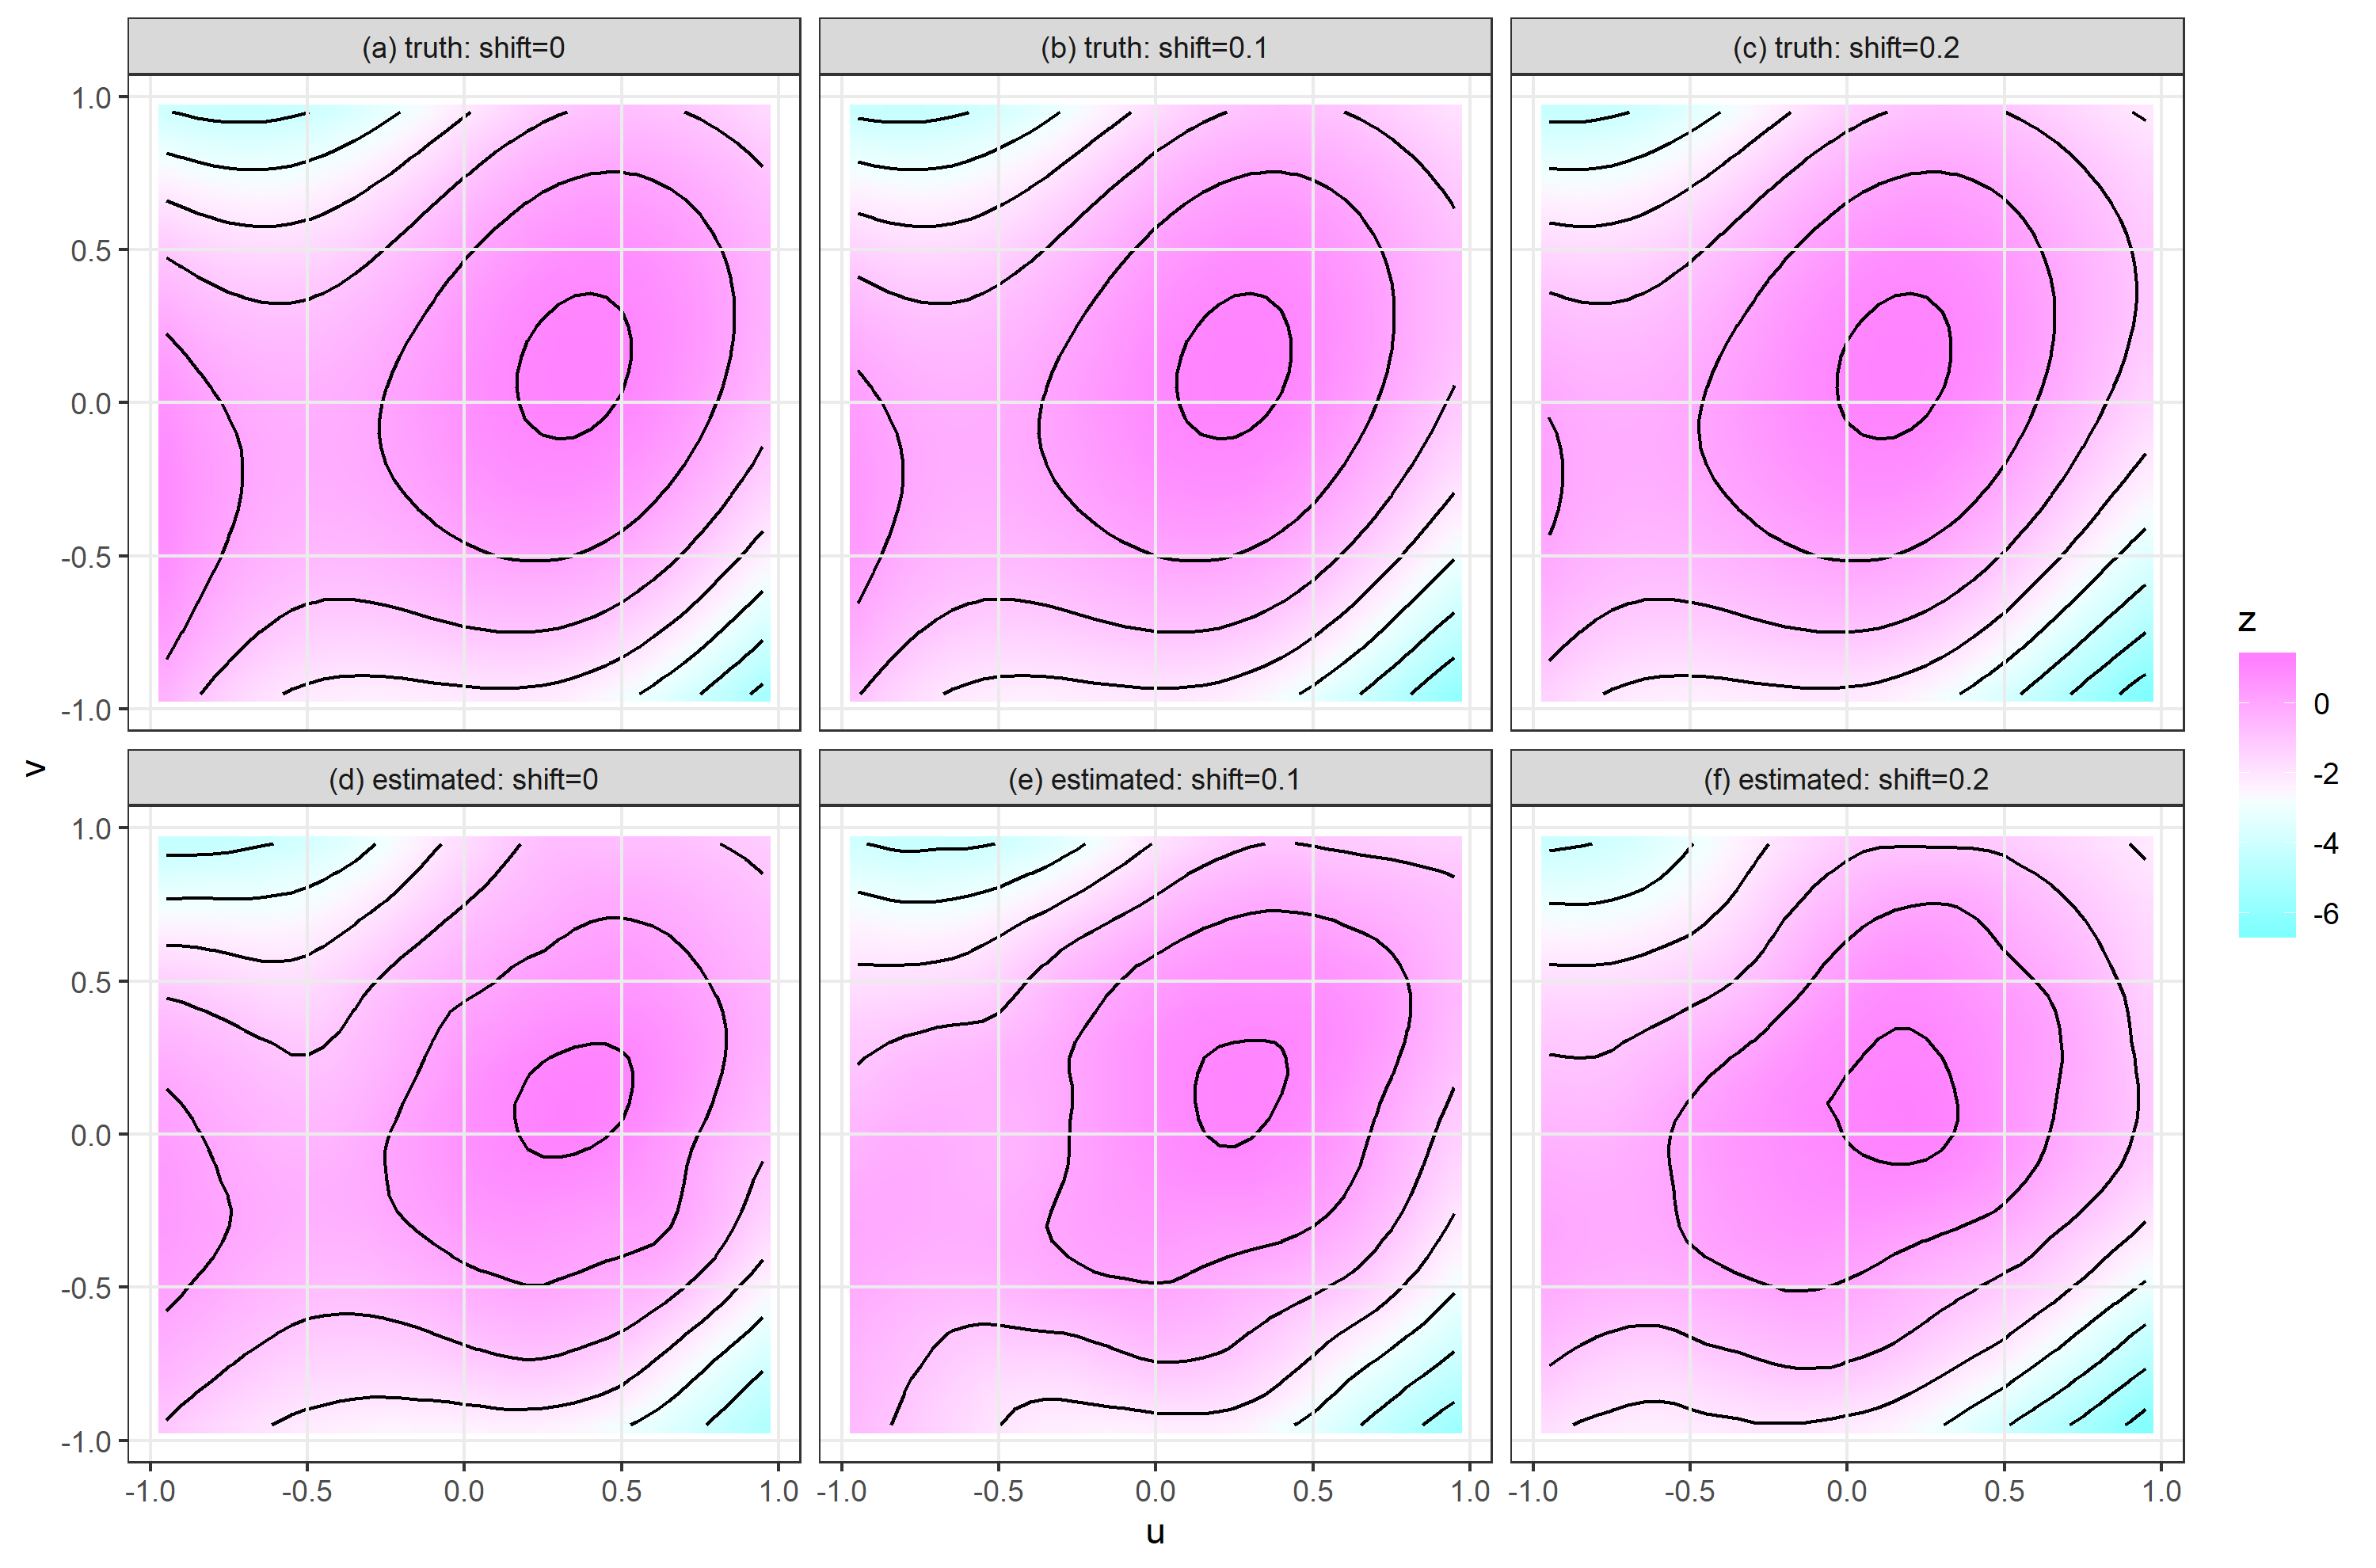
\includegraphics[width=\linewidth]{Figures/Chap3/TrueNEst.png}
		\caption{\textbf{Top}: Patterns used in nonlinear risk pattern simulations. ``shift" stands for the shifting amount of the whole pattern to left; \textbf{Bottom}: Estimated spatial risk patterns using our proposed model (in (\ref{stramodel})).}
		\label{fig:1}
	\end{figure}
	
	Using our proposed generalized additive model in (\ref{stramodel}), we are able to estimate the risk patterns at each time point. One simulation study is used to assess the performance of the stratified LOESS smoothers. 3 time points are set up with time-varying geospatial risk patterns where shift amounts are 0, 0.1 and 0.2, respectively. The 3 plots in the bottom of Figure \ref{fig:1} show the estimated risk patterns at each time point. From the plots, it is shown that the proposed time-specific LOESS smoothers are capable of recreating each of the time-specific geospatial risk patterns.
	
	Several simulations are conducted with 2 time points in total. Under $H_0$, we assume homogeneous underlying spatial effects ("shift=0") at both time points.  For simulations under $H_1$, "shift=0" is used for Time 1 and a shifted pattern is used for Time 2. The amount of shift indicates extremity of deviation from $H_0$, hence greater shift amounts should be detected with greater statistical powers. 
	
	Empirical powers are defined as the proportion of simulations in which $H_0$ is rejected. A level of significance of $\alpha=0.05$ is used. In each simulation scenario, simulation is repeated 500 times and $N_{perm}=1000$. As a comparison, we also consider ANOVA tests for temporal homogeneity in the above simulation settings when a naive parametric form of spatial effects is assumed. Specifically, consider Model (\ref{mod:ano1}) and and test $H_0: \beta_5=\beta_6=\beta_7=0$ using a permutation version of the F test. A permutation strategy is used in order to maintain a correct type I error. Specifically, for each simulated dataset, the permuted ANOVA procedure simply compares the observed F statistic and permuted F statistics, where the permuted F statistics are calculated using dataset with randomly permuted time labels. Also, the \emph{mgcv} package offers a class of stratified thin-plate regression splines and corresponding ANOVA tests. We applied this test as well for comparison. The resulting powers are shown in Panel (a) of Figure \ref{fig:twobtwo}.
	
	\begin{equation} \label{mod:ano1}
	E(Y_{ij}) =\beta_0+\beta_1u_{ij}+ \beta_2v_{ij}+\beta_3 t_{ij} + \beta_4 u_{ij} v_{ij} + t_{ij}(\beta_5u_{ij}+ \beta_6v_{ij}+\beta_7  u_{ij} v_{ij}) 
	\end{equation}
	
	To assess the performance of the PMSD test on datasets with more than 2 time points, we create datasets with 4 time points. No shift is used at time point 1 and a shift amount $S$ is applied at time point 4. For time 2 and 3, we used uniformly spaced shift amounts $S/3$ and $2S/3$. The resulting powers under these settings are shown in Panel (c) of Figure \ref{fig:twobtwo}. 
	
	\begin{figure}[h]
		\centering
		\includegraphics[width=\linewidth]{Figures/Chap3/Plot2b2XL1.png}
		\caption{\textbf{Panel (a)}: Power vs. shift amount based on 500 simulations at each shift value. Increasing rejection proportion could be observed. Type I error (rejection proportion at shift=0) is 0.046 for permutation test on F statistic, 0.032 for ANOVA F test based on thin-plate regression splines and 0.056 for PMSD test. The proposed PMSD test has the highest power in detecting temporal heterogeneity and permutation test based on parametric models renders the lowest power; 
			\textbf{Panel (b)}: Power vs. sample size based on 500 simulations at each sample size, given shift=0.15. Power increases along with sample size and approaches 1 near a sample size of 350 observations per time point; 
			\textbf{Panel (c)}: Power vs. shift amount at time point 4 based on 500 simulations at each shift value. Increasing rejection proportion (or greater power) could be observed. Type I error (rejection proportion at shift=0) is 0.062 for permutation test on F statistic, 0.018 for ANOVA F test based on thin-plate regression splines and 0.042 for PMSD test. Similarly, our proposed PMSD tests have better performance in power in detecting temporal heterogeneity;
			\textbf{Panel (d)}: Power vs. multiplier $\tau$ in (\ref{eq:paratruth}) based on 500 simulations at each value of $\tau$. As expected, classical ANOVA F test performs better in terms of power since it is the ``correct" test hence most powerful. In the meanwhile, the performance of PMSD is close to the F test.}
		\label{fig:twobtwo}
	\end{figure}
	
	The Monte Carlo results presented in Figure 2 for the PMSD test utilize a uniformly distributed $20\times 20$ grid on the entire $2\times 2$ map. Although a $20\times 20$ grid is seemingly sufficient for the risk patterns in the simulation studies we performed, we suggest a grid that is dense enough in order to sufficiently evaluate local behaviors. 
	% To explore the sensitivity of PMSD tests to the density of grid, we considered the impact of grid density on the performance of PMSD tests. Using simulation study, we evaluated a variety of grid densities for the PMSD test given a fixed shift amount 0.1. The corresponding power curve for each grid selection method is shown in Figure \ref{fig:gridpower}. These results suggest that too sparse a prediction grid hampers power, but simply choosing a higher density grid does not increase power to 1 (as it shouldn't). Note the distribution of the observed locations is uniform as well, 2 curves do not differ by much. 
	
	In addition to the grid density, another decision to make when performing PMSD tests is grid selection strategy. Intuitively, one might choose uniformly distributed locations on the entire map or the observed locations within the dataset. Since the MSD statistic is defined as the mean of squared differences at a chosen set of locations, the pattern of the grid intrinsically defines the weights assigned over the map. For temporal heterogeneity detection, a uniform grid will place equal weights on all areas of the map while observed locations put higher weight on areas with denser observations. As a simple example, given a risk pattern where temporal variation exists in one area of the map, using more points in the varying area in the grid for PMSD tests would result in higher power since the test would be weighted more heavily in the varying area due to the grid design. 
	
	To assess the impact of grid selection strategy on power, we performed simulation studies in 2 more scenarios. In Scenario 1 (shown in the plots in the top row of Figure \ref{fig:simuV2}), we use the same pattern as the previous simulations with 2 time points where we use "shift=0" for Time 1 and "shift=0.1" at Time 2. The observations are designed to be uniformly distributed on the map. We vary $N_g$, the number of locations used in the grid, to explore the impact of grid density on power. For each $N_g$ value, we simultaneously chose $N_g$ random locations from a uniform $20\times 20$ grid on the map and another random collection of $N_g$ locations from the observed location set. Using the 2 sets of locations, PMSD tests were performed in order to assess the impact of grid selection strategy on power. In Scenario 2 (bottom row of Figure \ref{fig:simuV2}), we use another design of spatial risk surface which has 2 high risk areas. We use the pattern at Time 1 and mitigate the risk by 30\% in one of the high risk areas at Time 2 to create temporal heterogeneity. In this setting, observations are designed to be denser in high risk areas. We performed similar grid selection and testing procedures to those of Scenario 1 and compared power with respect to grid density and selection strategy. From the empirical power results, the denser grids tend to render higher power, which is reasonable since local variations are more likely to be detected with more evaluated locations. In Scenario 1, tests using observed locations yield slightly higher power than those using uniform grids. This result could be explained by higher precision in spatial effects estimation at observed locations. The performance of tests using observed locations is much better than that of tests using a uniform grid in Scenario 2, which is as expected since more locations in time-varying areas are evaluated by MSD statistic, resulting in greater weights in the areas when the test is performed. 
	
	\begin{figure}[h] 
		\centering
		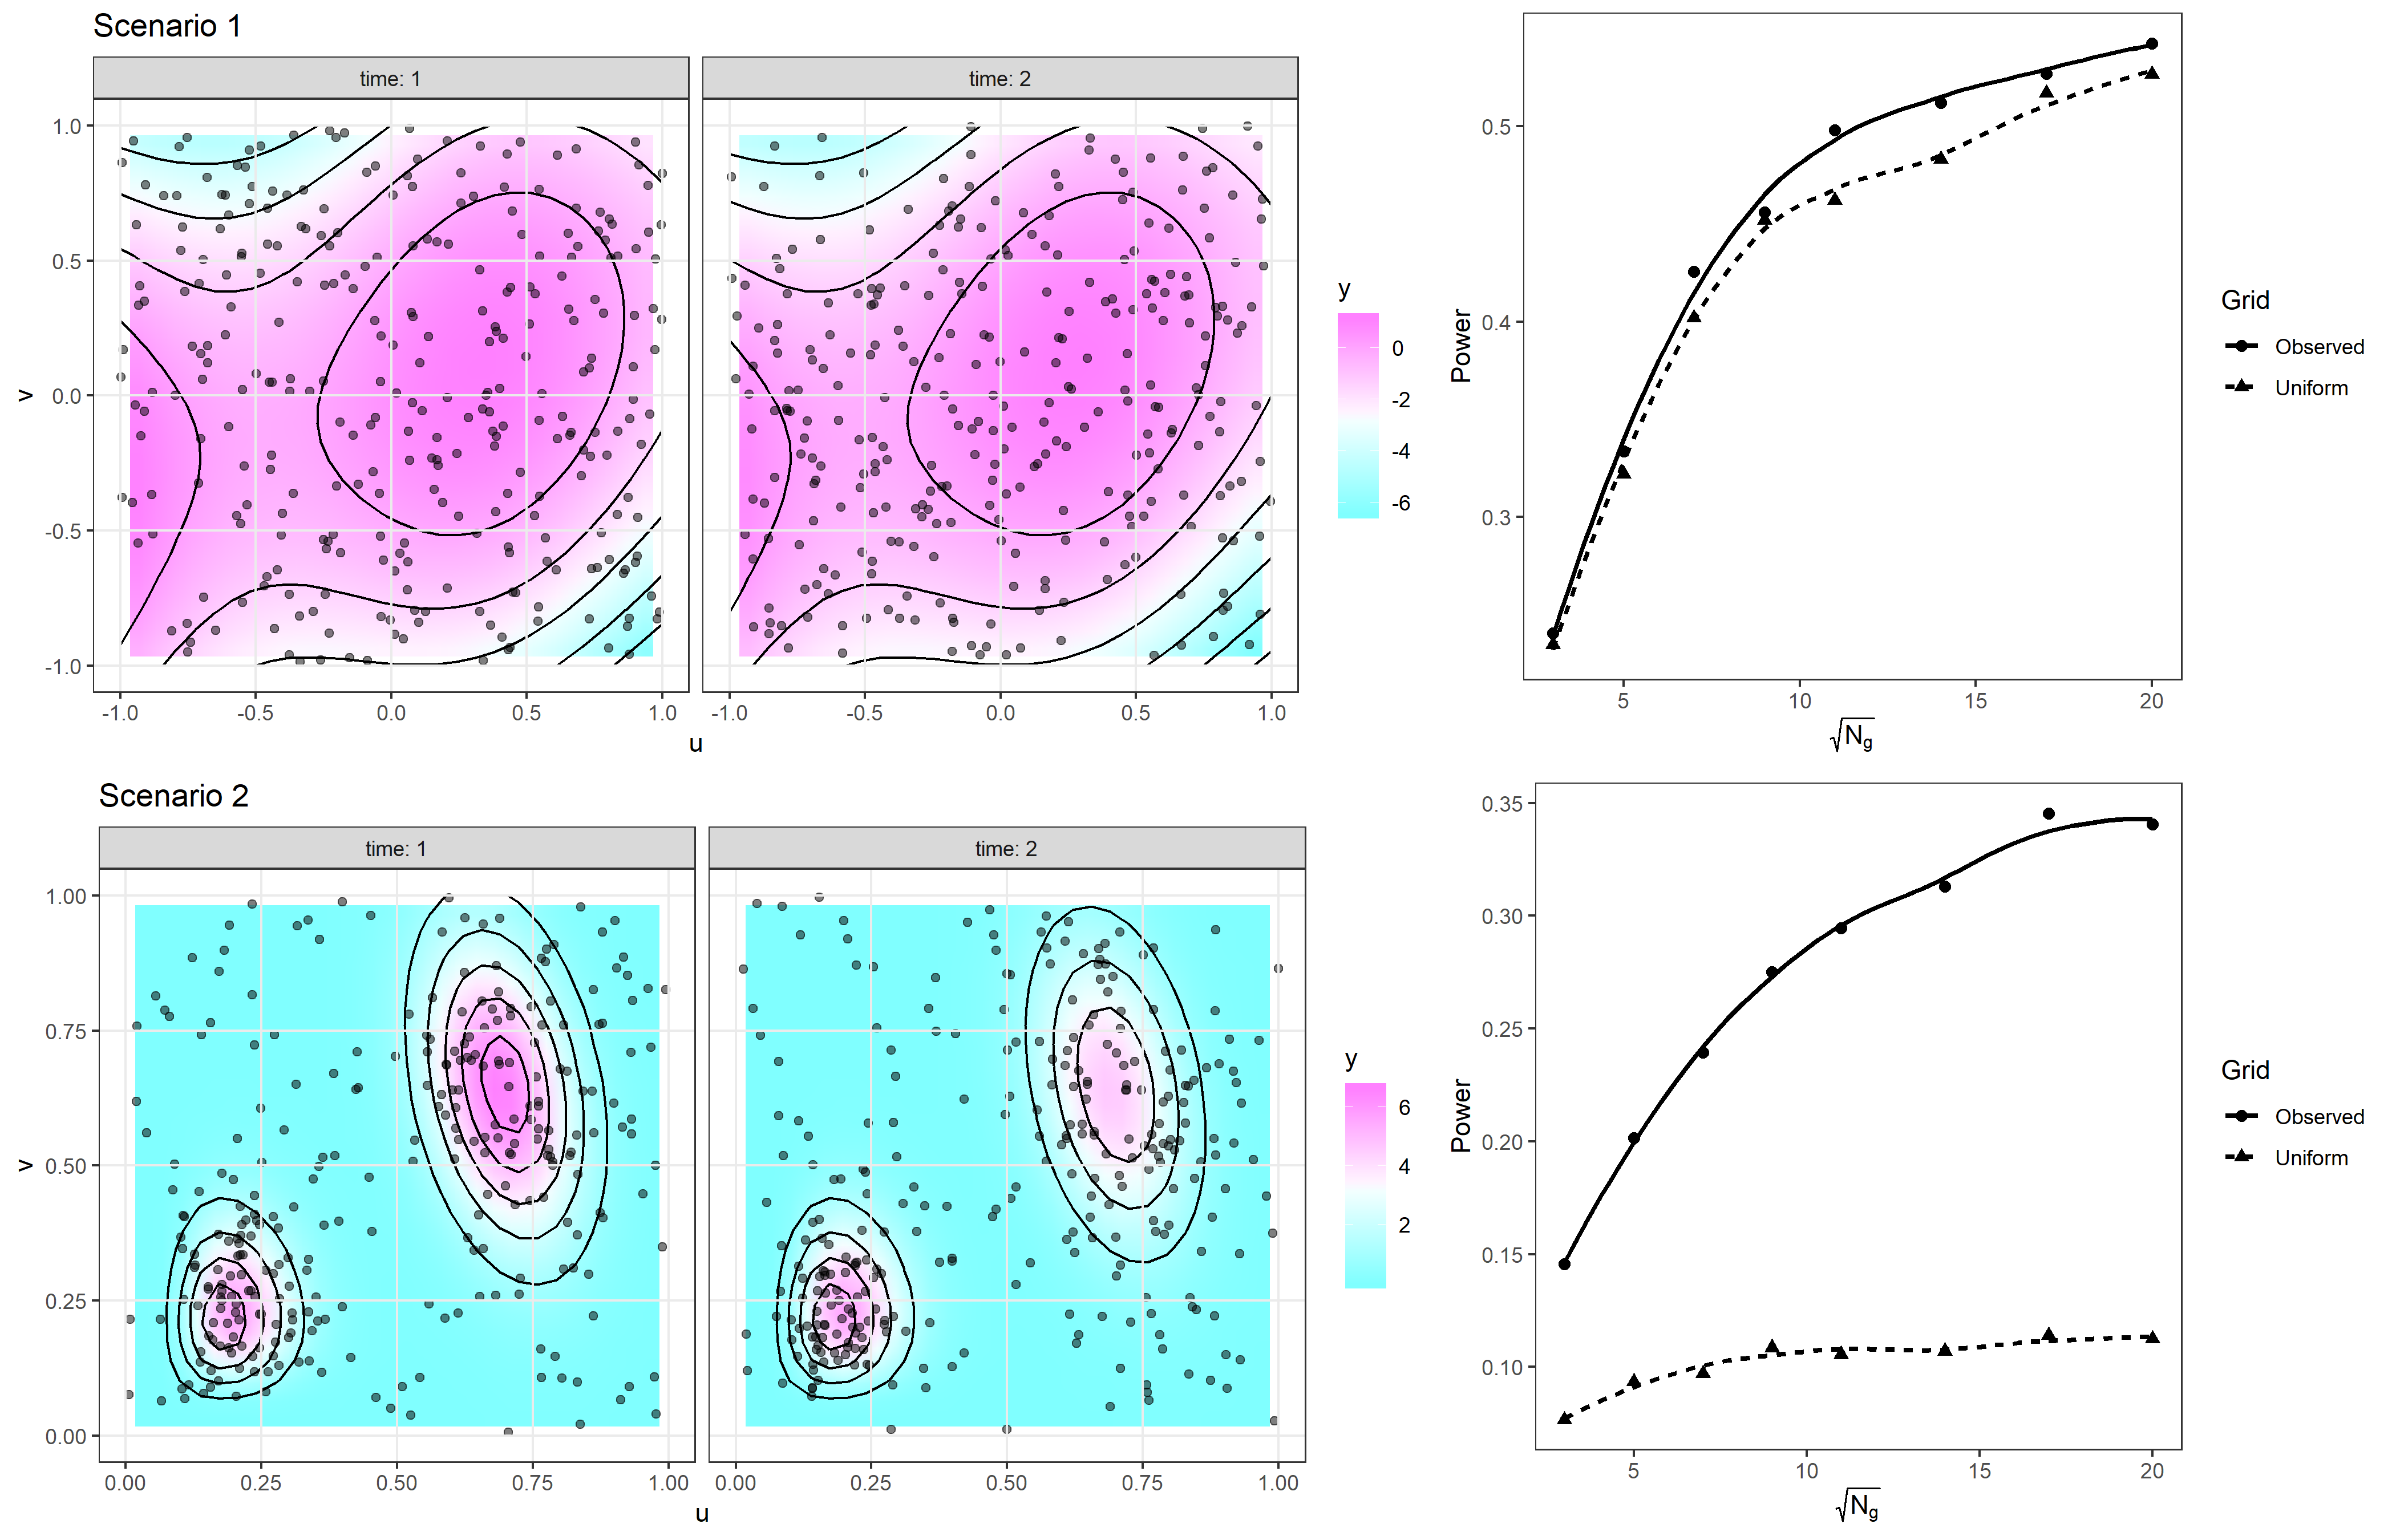
\includegraphics[width=\linewidth]{Figures/Chap3/gridc1234SNR.png}
		\caption{\textbf{Top}: Geospatial risk patterns at Time 1 and 2 with observed locations in Scenario 1 and corresponding power v.s. density curves for PMSD tests using uniform and observed grids. \textbf{Bottom}: Geospatial risk patterns at Time 1 and 2 with observed locations in Scenario 2 and corresponding power v.s. density curves for PMSD tests using uniform and observed grids.}
		\label{fig:simuV2}
	\end{figure}
	
	\subsection{Simulation studies with linear underlying patterns}
	
	In the previous Monte Carlo studies, we assume nonlinear underlying spatial patterns, as is shown in Figure \ref{fig:1}. In these situations, our proposed PMSD test outperformed a permutation version of the F test, as is expected. In this section, we conduct a simulation study where the true underlying spatial risk patterns are created using a linear function of longitude and latitude and compare the finite sample behavior of the PMSD tests and the optimal F tests.  Specifically, data were generated using the following model:
	\begin{equation}
	y_{ij}=-2+3u_{ij}-3v_{ij}+u_{ij}v_{ij}+\tau t_{ij}(2u_{ij}+2v_{ij}+u_{ij}v_{ij}+1)+\epsilon_{ij}.
	\label{eq:paratruth}
	\end{equation}
	
	In the above model, values from 0 to 0.16 are chosen to be $\tau$. $\epsilon_{ij}$'s are $i.i.d.$ random errors from a standard normal distribution. We apply both a classical ANOVA F test of the space-time interaction terms (a correctly specified model) and the PMSD test. Using a similar strategy as previous sections, we compare the performance of the 2 classes of tests and plot the results in Panel (d) of Figure \ref{fig:twobtwo}. Both tests yield correct type I errors while the ANOVA test yields slightly higher power. However, the increased power comes at a high cost, as the inflexible parametric model does not perform as well if the underlying risk pattern is more realistically nonlinear.
	
	\section{Application to birth defects study in Massachusetts}
	
	In this section we use our proposed methods to analyze the data achieved by the previously introduced MBDR study. Given the severity of PDA, it is of interest to determine if space-related risk factors place infants at increased PDA risk. Generalized additive models with a bivariate smoother incorporated, such as the model in (\ref{mod:orig}), estimate cross-sectional geospatial risk patterns with adjustment for other potentially relevant factors including maternal age, adequacy of prenatal care (measured by the Adequacy of Prenatal Care Utilization Index), maternal race, maternal education level and number of siblings, as is applied in  \cite{girguis2016maternal}. 
	
	Beyond the analysis of cross-sectional data in each year, we further aim to investigate the existence of variation in spatial risk patterns over time. We applied our methods on data collected in 2003, 2006, and 2009. Available sample sizes for the three years are 1082, 969, and 877, respectively. Corresponding numbers of PDA cases are 111(10.3\%), 90(9.3\%) and 60(6.8\%). The geographic distribution of the observations are shown in the top row of Figure \ref{fig:MAdist}. With adjustment for maternal age, adequacy of prenatal care, maternal race, maternal education level and number of siblings, the estimated geospatial risk patterns are shown in the bottom row of Figure \ref{fig:MAdist}. PMSD tests were performed to assess heterogeneity over the 3 years. The results are shown in Figure \ref{fig:MApvalues}. 
	
	\begin{figure}[h]
		\centering
		\includegraphics[width=\linewidth]{Figures/Chap3/obnest201904.png}
		\caption{\textbf{Top}: Distribution of PDA cases (red) and controls (black) over selected years. Sparsity in western Massachusetts reflects lower population density; \textbf{Bottom}: Estimated geospatial risks for each year with adjustment for relevant variables. Values presented are estimated log odds ratios. The solid lines on the estimated patterns indicate areas with significant nonzero log-odds using $\alpha=0.05$. The significance is determined by a permutation test described in \cite{webster2006method} The idea of the test is to randomly permute the locations of the observations and recalculate the log-odds for M times in order to achieve a point-wise reference distribution of log-odds at each point on map. The significant areas contain points where the estimated log-odds is outside of the 95\% confidence interval constructed by the reference distribution. The test is applied using R package \emph{MapGAM}. \citep{bai2019mapgam} According to the estimated surfaces, southeast Massachusetts has potentially significant high PDA risk in 2006 but low risk in both 2003 an 2009. In addition, a high PDA risk appears at central-southern Massachusetts in 2009.}
		\label{fig:MAdist}
	\end{figure}
	
	\begin{figure}[h]
		\centering
		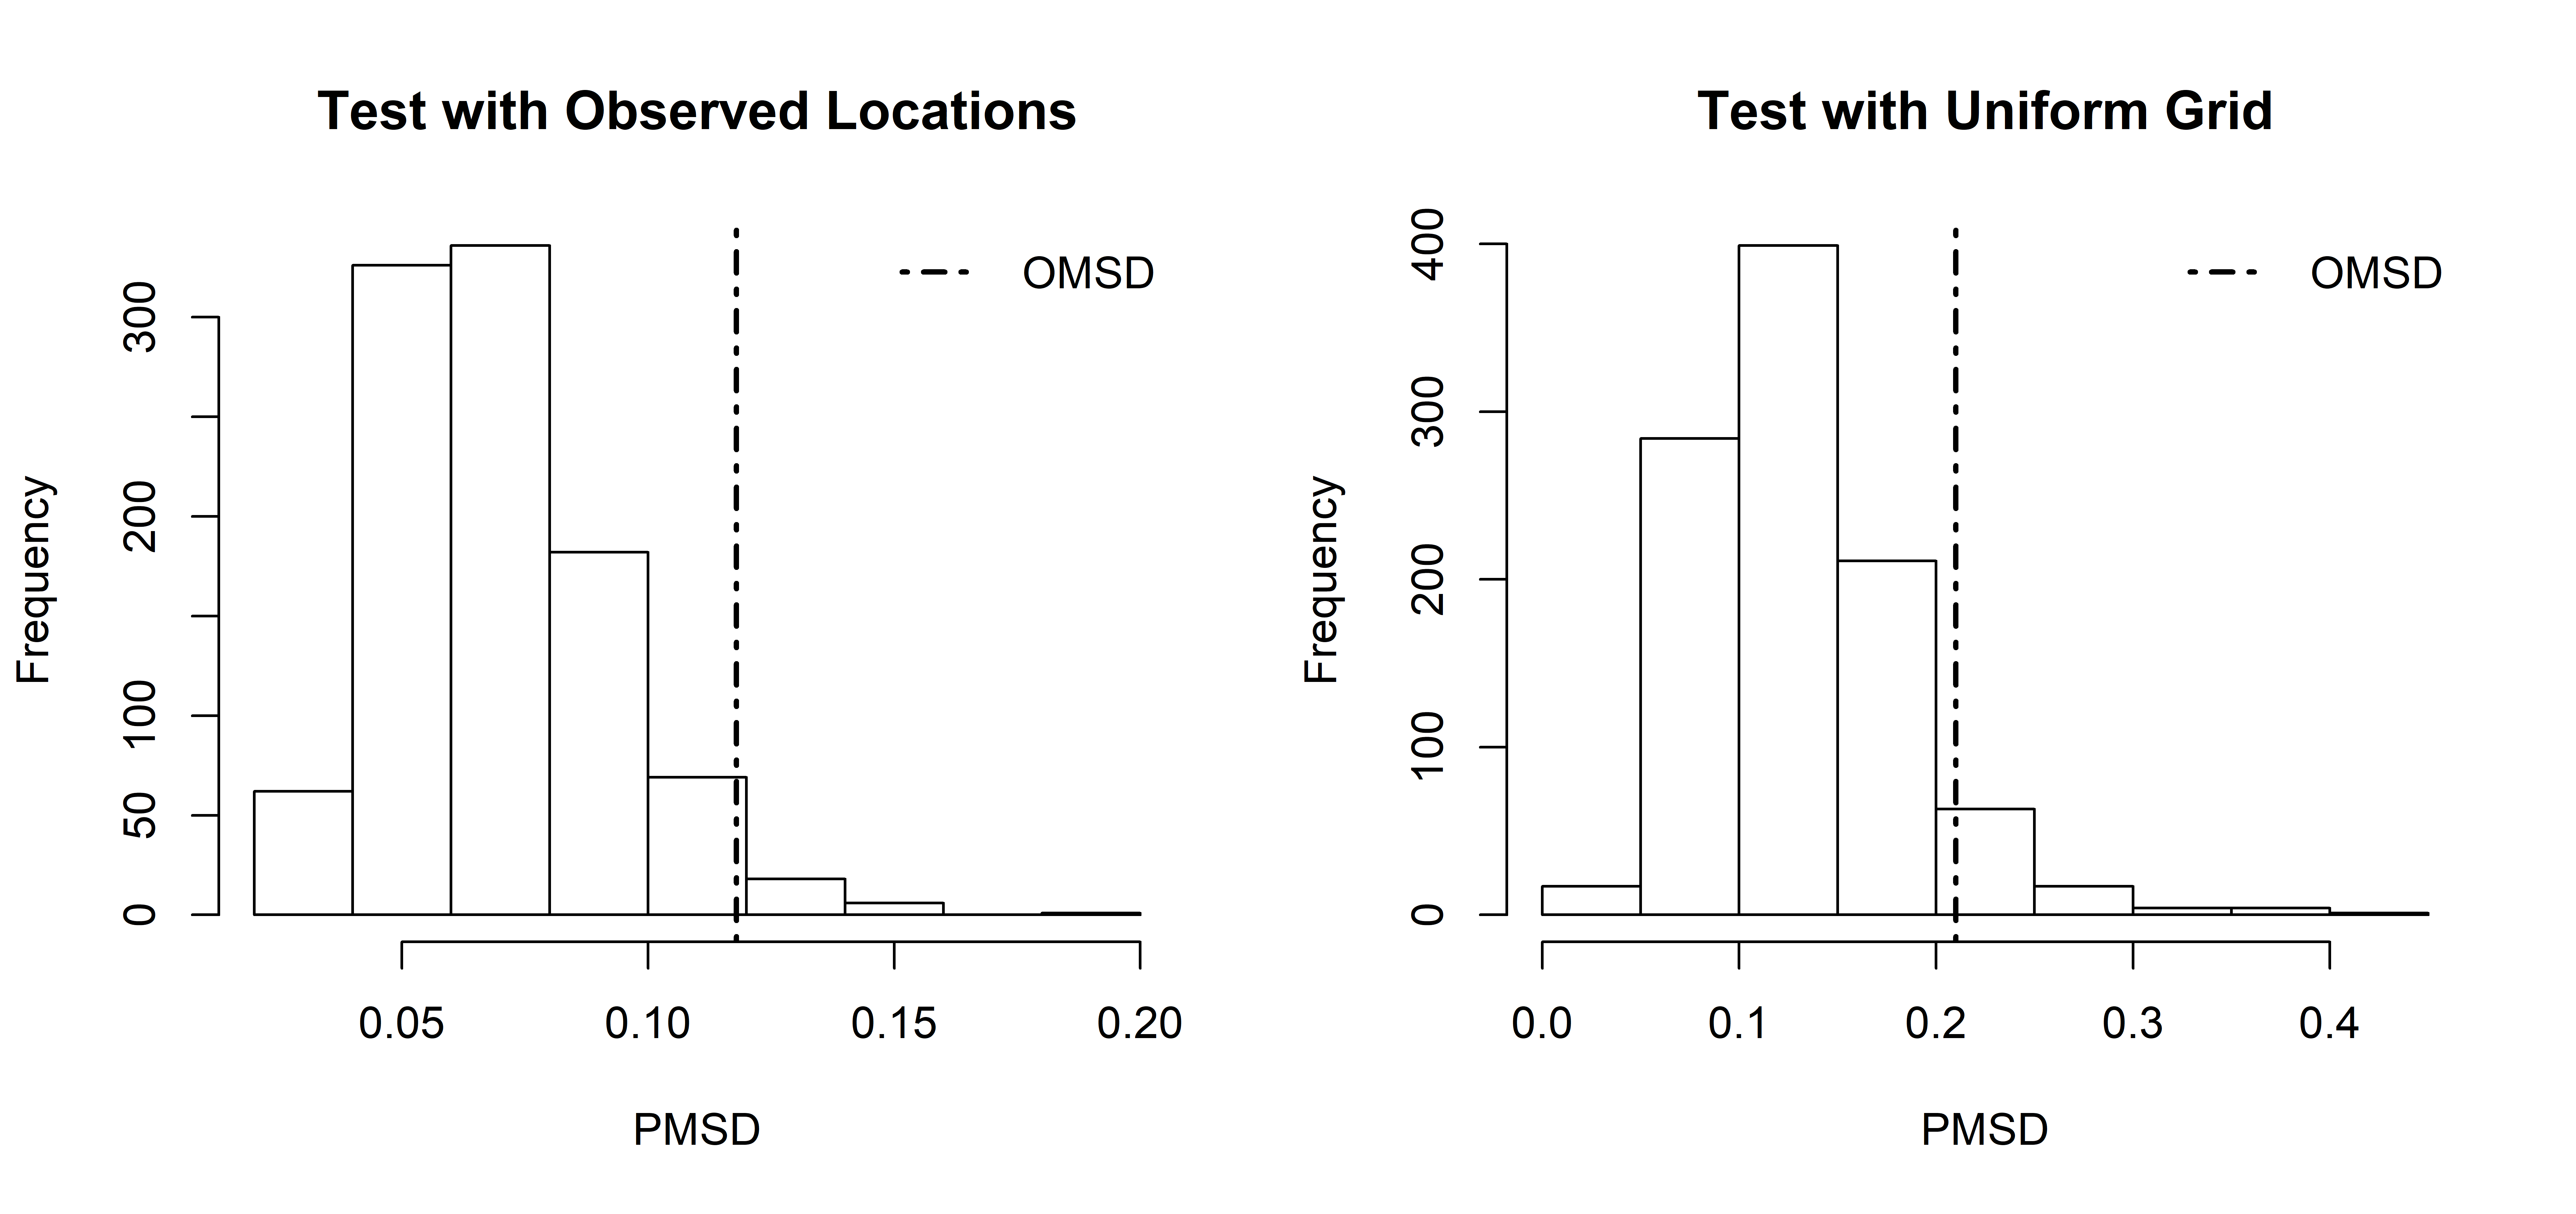
\includegraphics[width=0.9\linewidth]{Figures/Chap3/AppRes.png}
		\caption{Histograms of PMSD values using 2 test location selection strategies with vertical lines indicating the value of OMSD. The p-values are 0.029 using observed locations and 0.069 using a uniform grid on the Massachusetts map.}
		\label{fig:MApvalues}
	\end{figure}
	
	From the estimation in Figure \ref{fig:MAdist}, potential temporal heterogeneity of geospatial PDA risk is observed by visual inspection. To formally determine if the spatial risk changes over the period, we apply our proposed PMSD test and the resulting p-value is $0.028$, indicating potential time-varying and space-related factors for PDA risk other than the adjusted ones in the model over the 7 years from 2003 to 2009. Note that since the PMSD test aims to find any temporal change in the geospatial risk patterns, the detected heterogeneity could be a result of either a change in the overall level of PDA rate at each time point or a change in the spatial disparity patterns of PDA risk.
	
	The presented analysis utilizes all observed locations as evaluation points. The PMSD test utilizing a uniform grid on the Massachusetts map renders a greater p-value ($=0.069$) than the one using the observed locations (consistent with our previously presented simulation results). Corresponding PMSD and $\emph{OMSD}$ values are plotted in Figure \ref{fig:MApvalues}. As discussed previously, the choice between the two grid choice strategies should also take into account the scientific goals of the study. The PMSD test using observed locations places weights that are roughly proportional to the population (under a simple random sample) while the PMSD test using a uniform grid equally weights all areas of Massachusetts. 
	
	\section{Discussion}
	In this study, we brought in time-stratified kernel smoothers to the generalized additive model framework for estimation of time-specific geospatial disease risk patterns. Based on the proposed GAMs, we further formalized a permutation test for temporal heterogeneity of smoothed spatial risk effects.
	
	Using simulation studies, we showed that our proposed PMSD test performed substantially better than the other 2 competitors in detecting underlying temporal heterogeneity given a specific nonlinear spatial pattern. Even when the difference between spatial risk patterns was not clearly noticeable by visual inspection, the proposed procedure yielded acceptable power. In situations with parametric spatial risk patterns, a correctly specified parsimonious parametric ANOVA F test only slightly outperformed the PMSD test. We did assume smoothness of the surface in the presented simulations as well as smooth shifts over time as there would likely not be abrupt shifts in the spatial or temporal patterns for the birth defect data that motivates our methodology.  We do, however, acknowledge that non-smooth patterns can exist and differential changes in hot spots may arise. In additional simulation studies, not presented here, we considered the performance of our methods in the setting of abrupt changes in the response surface. We found that our model managed to render reasonably good estimation although the estimated pattern is not as accurate at the areas where the risk changes dramatically, which is not surprising since the smoothness assumption is violated. We also found that the type I error rate of our proposed PMSD test was maintained and that relative power benefits compared to the F test were also maintained in this setting. 
	
	Straightforward extensions of the proposed methods may be of interest in particular settings. For instance, if multiple contiguous time points are assumed to share one common spatial risk pattern, these time points could be grouped as one strata. Thus the stratified smoothers and corresponding PMSD tests are naturally applied to multiple time stratas, rather than to all time points. A similar strategy could be adopted for cases with continuous time, where smoothers could be stratified at separate time intervals. Also, when researchers wish to investigate heterogeneity in geospatial risk patterns over a categorical factor other than time, such as sex or discretized age, the proposed methods remain applicable. 
	
	The proposed PMSD test considers a global test for temporal homogeneity of spatial effects, as opposed to identification of specific local area differences. This is a natural first step in the identification of changing spatial patterns over time. Note that when temporal variation of geospatial risk pattern exists merely localized while the grid for MSD statistics is designed on the entire map, the power may suffer from the inclusion of geographic locations where the risk does not vary over the time period in MSD statistic. One next step, as we have done in the MBDR analysis for cross-sectional data analysis, is to highlight areas with differential risks. This is akin to first establishing the existence of main effects then further investigating effect modification. 
	
	Other than what is proposed in this work, smoothing with respect to time seems to be an intuitive way to model space-time data, but naively including time in smoothing terms is questionable. Using two separate smoothing terms in an additive way, one for spatial effects and another for time effects, fails to model time-space interaction while using a 3-way smoother including longitude, latitude and time offers flexible smoothing but suffers from anisotropy and potentially sparseness. The proposed procedures make no assumption on temporal correlation and put no restriction on how geospatial effects pattern varies. Some might be concerned about loss of efficiency due to the flexibility. We would argue that for large data sets, which is frequently the case in epidemiology studies, efficiency is maintained at each time point. As supporting evidence, Panel (d) of Figure \ref{fig:twobtwo} shows close performance between PMSD tests and the optimal ANOVA F-tests under parametric spatial risk patterns, indicating little efficiency loss.
	
	For statistical inference on smoothing components in GAMs, an approximate F-test was introduced by \cite{hastie1990generalized}. However, simulation studies showed that this approximate F-test renders inflated type I error in \cite{young2011generalized}. According to simulation results of the approximate F-test (not shown in this manuscript) on our simulation problem, inflated type I errors are observed as well. However, due to its efficiency potential, we will explore calibrating methods for this class of approximate F-tests in our future work. 
	
	An intuitive Bayesian counterpart of the stratified smoother could be a time-stratified Gaussian process where one process is set up at each time point with or without shared hyperparameters. A stratified Gaussian process only requires modification of the likelihood. This stratification does not require a specific time-space covariance structure since no specific temporal correlation is assumed. Based on this class of models, temporal heterogeneity in spatial patterns can potentially be tested using the Bayes factor.\citep{kass1995bayes} While we appreciate the Bayesian framework in geospatial modeling, many health researchers are not closely familiar with Bayesian methods.  In contrast, local linear regressions may be more intuitive and accessible to nonstatisticians. In particular, tuning a span size that is understandable as the proportion of data utilized in the local window of smoothing, is more straightforward than choosing hyperparameters in covariance structures of a Gaussian process. In addition, GP models tend not to scale well with respect to computation. In contrast, the time-stratified generalized additive models proposed here are computationally cheap and easily scale to large data sets. We compared model fitting time between GP models and GAMs using the R package \emph{spBayes} \citep{Finley2007, Finley2015} and R package \emph{gam} \citep{hastie1990generalized} respectively. GP models were roughly 20 times more computationally expensive when compared to GAMs for $N=100$. Computation times were roughly 200 times greater for $N=300$, 500 time greater for $N=500$ and 1000 greater for $N=700$, indicating a disadvantage of GP models with respect to scalability. Given these potential advantages, we view the proposed procedure as providing another useful tool to spatial epidemiologists.
	
	%In this paper, we assume simplistic homogeneous or heterogeneous risk patterns for our simulations, as well as independence over time conditional upon all adjustment covariates. Hence our method tests temporal homogeneity without assessing temporal correlation, and assumes no unmeasured confounding.
	
	One key assumption we made in this paper is mutual independence of all observations. That is to say, cross-sectional studies over multiple time points, rather than longitudinal studies, are discussed. Since longitudinal studies where individuals have multiple measurements over time are increasingly prevalent, in the future, we plan to further generalize stratified smoothers and investigate the performance of the PMSD tests on longitudinal data.
	


%%% Local Variables: ***
%%% mode: latex ***
%%% TeX-master: "thesis.tex" ***
%%% End: ***
